\chapter{无向图模型}
\label{chap:pgm-undirected}

图像分割要为多个相邻像素同时分配标签。相同物体中的邻近像素通常倾向于采用相同标签，这种关系可以直接按空间邻接建模：为相容配置赋予较高权重，再考察观测一组标签后，其他区域之间还保留哪些依赖。第~\ref{chap:pgm-directed}章的有向模型按父子方向组织条件分布，本章则以对称的局部相互作用和路径阻断组织联合分布。

路径阻断说明哪些区域在给定观测后条件独立，局部函数乘积则给出各个标签配置的概率。本章先建立成对、局部和全局三种Markov性质，再证明团上的局部乘积怎样表达这些关系。由独立性反推乘积分解时，零概率配置会影响所能约束的局部组合；连续变量还涉及密度的积分与版本。因此，各个方向的推理将随相应的正性、测度和归一化条件一同说明。

\section{无向图模型的定义}
\label{sec:pgm-undirected-definition}

用$X_1,\ldots,X_4$表示四个相邻区域的二值标签，并将它们按空间邻接连成环：$1$与$2$、$2$与$3$、$3$与$4$、$4$与$1$相邻。环上的边记录区域之间的直接局部相互作用。后文采用这个人工模型计算条件概率，并通过改变配置的支持集，检查分离关系与严格正性条件的作用。

本章采用有限简单无向图$\mathcal G=(V,E)$，节点集为$V=\{1,\ldots,d\}$，并排除自环与重边。邻接约定参见\BookSectionRef{sec:graph-theory-local-relations}{第一卷“数学准备”的图局部关系小节}。与$i$直接相连的节点组成邻居集合：
\[
  N(i)=\{j\in V:\{i,j\}\in E\}.
\]
每个节点$i$对应标量随机变量$X_i$，小写$x_i$表示其取值。将节点集合$A\subseteq V$中的变量组成向量，记为$\bm{X}_A$，其取值记为$\bm{x}_A$。节点编号描述图中的位置，状态描述变量的结果，例如$1\in V$指定节点，$x_1=0$指定该节点的一次取值。

从节点$i$沿现有边走到$j$，并使每个节点只出现一次，所得序列称为\term{路径}（path）。彼此有路径可达且无法继续扩大的节点集合称为\term{连通分量}（connected component）。若只保留节点集合$D$及其内部全部原有边，就得到\term{诱导子图}（induced subgraph）$\mathcal{G}[D]$。删除观测节点后检查剩余连通分量，将是无向分离检测的主要操作。

局部函数若涉及多个变量，需要说明哪些变量组合由图允许。任意两个不同节点都相邻的非空集合称为\term{团}（clique），单节点集合也属于团。一个团若加入任何其他节点都会破坏这一性质，就称为\term{极大团}（maximal clique）；这里的极大性针对包含关系。图~\ref{fig:pgm-undirected-cliques}左侧的环有四个二节点极大团，三节点集合都缺少一条边；右侧的两个三角形分别给出极大团$\{1,2,3\}$与$\{3,4,5\}$。

\begin{figure}[htbp]
  \centering
  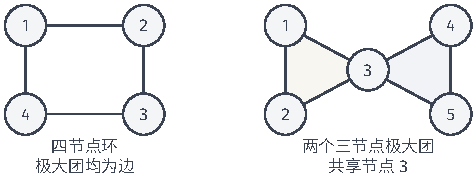
\includegraphics[width=80.652mm]{figures/06-probabilistic-graphical-models/01-representation/tikz/pgm-undirected-cliques/figure.pdf}
  \caption{无向图中的团与邻接。左图的四条边分别构成极大团，整个环因缺少对角边而不构成团；右图的两个三角形为极大团，共享节点$3$。无向线段表示邻接，节点编号对应随机变量下标。}
  \label{fig:pgm-undirected-cliques}
\end{figure}

观察一组节点后，两侧之间若已没有剩余路径，就用条件独立描述两侧的概率关系。采用这种语义的模型称为\term{无向图模型}（undirected graphical model），也称\term{Markov随机场}（Markov random field, MRF）或Markov网络。第~\ref{sec:pgm-undirected-global-independence}节将对任意节点集合正式陈述这项全局要求。

同一张无向图可以配上不同的局部函数，得到不同的分布。图规定相容分布必须遵守的独立性，数值参数则决定相邻变量实际具有多强的依赖，也可能产生额外独立性。无向边首先描述概率相互作用，干预后的分布需要额外的因果建模语义。这里采用的分离与Markov语义见无向图模型的标准表述\scite{pgm-lauritzen1996}。

\section{无向图的局部独立性}
\label{sec:pgm-undirected-local-independence}

在四节点环中，可以先检查缺少对角边的两个节点，也可以检查一个节点与全部非邻居的关系。这两种查询分别给出成对和局部Markov性质。它们涉及的独立侧和条件侧不同，后文将说明怎样由这些局部要求恢复集合之间的全局独立性。

\subsection{成对Markov性质}
\label{sec:pgm-undirected-pairwise}

两个非邻接节点$i,j$仍可能经其他节点相连，消去中间状态后也可能相关。成对Markov性质将其余节点全部给定，使间接连接受到屏蔽，再要求这两个非邻接变量条件独立。

\begin{definition}[成对Markov性质]
  \label{def:pgm-undirected-pairwise}
  联合分布$p$相对于$\mathcal{G}$满足\term{成对Markov性质}（pairwise Markov property），是指对每一对不同且不相邻的节点$i,j$，都有
  \begin{equation}
    X_i\perp X_j\mid\bm{X}_{V\setminus\{i,j\}}.
    \label{eq:pgm-undirected-pairwise}
  \end{equation}
\end{definition}

四节点环中的非邻接对为$\{1,3\}$和$\{2,4\}$，对应的成对约束为
\[
  X_1\perp X_3\mid(X_2,X_4),
  \qquad
  X_2\perp X_4\mid(X_1,X_3).
\]
第一项同时以$X_2,X_4$为条件，这两个节点分别位于两条连接路径上。只给定$X_2$时，路径$1-4-3$仍然存在，结构尚未保证$X_1\perp X_3\mid X_2$。

对于离散变量，在$p(\bm{x}_{V\setminus\{i,j\}})>0$的条件配置下，二元条件概率应分为两个条件边缘的乘积，概率比定义也在这些事件上使用。零概率条件事件的版本不受同一比值规定。连续变量则采用条件密度或正则条件分布，等式按条件变量的分布几乎处处成立，其依据与离散单点的正概率条件不同。

成对性质便于按缺边列出约束，而集合查询还要同时处理多个变量。将一些已给定的变量移回未知侧会改变条件分布，因而从成对约束得到较大集合的独立性，需要相应的概率运算规则。后面的弱并与交性质将分别处理两种集合变化。

\subsection{局部Markov性质}
\label{sec:pgm-undirected-local}

从$i$到非邻居的每条路径，第一步都经过$N(i)$。因此，把全部邻居给定可以在图上阻断当前节点与其余节点的联系，局部Markov性质将这项屏蔽转换为条件独立要求。

\begin{definition}[局部Markov性质]
  \label{def:pgm-undirected-local}
  联合分布$p$相对于$\mathcal{G}$满足\term{局部Markov性质}（local Markov property），是指对每个$i\in V$，都有
  \begin{equation}
    X_i\perp\bm{X}_{V\setminus(\{i\}\cup N(i))}
       \mid\bm{X}_{N(i)}.
    \label{eq:pgm-undirected-local}
  \end{equation}
\end{definition}

给定某个节点集合后，若$X_i$与集合以外的其他变量独立，这个集合就称为$X_i$的\term{Markov毯}（Markov blanket）。满足局部Markov性质时，邻居集合$N(i)$是图保证的一个毯。图~\ref{fig:pgm-undirected-markov-blanket}以中心、邻居和远端节点三层展示这一结构：所有通向远端的路径都先经过邻居。

\begin{figure}[htbp]
  \centering
  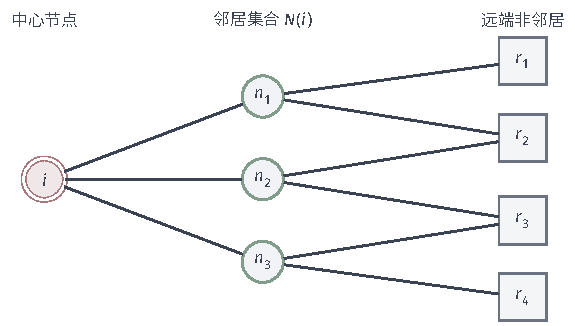
\includegraphics[width=97.402mm]{figures/06-probabilistic-graphical-models/01-representation/tikz/pgm-undirected-markov-blanket/figure.pdf}
  \caption{邻居集合构成的图上Markov毯。双边框圆为中心节点$i$，单边框圆为邻居$n_1,n_2,n_3$，方形为远端非邻居。实线均表示现存的无向边，中心到远端的每条路径先经过$N(i)$中的节点。}
  \label{fig:pgm-undirected-markov-blanket}
\end{figure}

在相应条件分布有定义的取值上，给定全部其他变量与只给定邻居得到相同的局部分布：
\begin{equation}
  p(x_i\mid\bm{x}_{V\setminus\{i\}})
  =p(x_i\mid\bm{x}_{N(i)}).
  \label{eq:pgm-undirected-blanket}
\end{equation}
该式说明邻居信息足以给出$X_i$的条件分布。特定分布$p$中的冗余参数可能允许更小的毯，例如某个邻居实际不改变局部分布时，可以将它省去。即使图含有环，邻居仍可屏蔽离开$i$的所有路径，因此这项结构保证保持成立。

\begin{figure}[htbp]
  \centering
  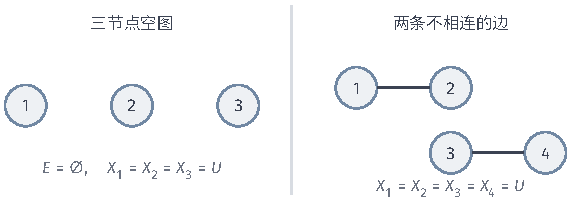
\includegraphics[width=96.686mm]{figures/06-probabilistic-graphical-models/01-representation/tikz/pgm-undirected-markov-counterexamples/figure.pdf}
  \caption{检验Markov性质逆向蕴含的两张图。各节点变量都等于同一个公平二值变量$U$，联合分布只有两个正概率配置。左侧空图满足成对性质而不满足局部性质；右侧两条不相连的边满足局部及成对性质而不满足全局性质。}
  \label{fig:pgm-undirected-markov-counterexamples}
\end{figure}

\begin{example}[成对性质不蕴含局部性质]
  \label{ex:pgm-undirected-pairwise-not-local}
  在图~\ref{fig:pgm-undirected-markov-counterexamples}左侧的三节点空图中，采用公平Bernoulli变量$U$，将三个节点都设为它的副本：
  \[
    X_1=X_2=X_3=U.
  \]
  空图的三对节点均不相邻，对应的全部成对约束是
  \[
    X_1\perp X_2\mid X_3,\qquad
    X_1\perp X_3\mid X_2,\qquad
    X_2\perp X_3\mid X_1.
  \]
  对第一项，在给定$X_3=u$的正概率事件下，两个未知变量也被确定为$u$。因此，对任意$u,a,b\in\{0,1\}$有
  \[
    \begin{aligned}
      p(X_1=a,X_2=b\mid X_3=u)
      &=\mathbf{1}\{a=u\}\mathbf{1}\{b=u\}\\
      &=p(X_1=a\mid X_3=u)p(X_2=b\mid X_3=u).
    \end{aligned}
  \]
  将$(X_1,X_2;X_3)$分别换为$(X_1,X_3;X_2)$和$(X_2,X_3;X_1)$，其余两项具有同样的指标函数乘积。三个成对约束由此全部成立。

  节点$1$的邻居集合$N(1)=\varnothing$，局部性质因而要求边缘独立$X_1\perp(X_2,X_3)$。比较全零状态的联合概率与边缘乘积，得到
  \[
    p\bigl(X_1=0,(X_2,X_3)=(0,0)\bigr)=\tfrac12
    \neq
    p(X_1=0)p\bigl((X_2,X_3)=(0,0)\bigr)=\tfrac14.
  \]
  两边分别为$1/2$和$1/4$，所以局部性质失败。分布只在$(0,0,0)$与$(1,1,1)$上为正，给定一个副本可以完全确定其他副本，而消去这个条件后，变量仍共同随$U$变化。这说明成对约束与无条件集合独立在当前支持集下有不同含义。
\end{example}

\begin{theorem}[局部Markov性质蕴含成对Markov性质]
  \label{thm:pgm-undirected-local-to-pairwise}
  设$\mathcal{G}=(V,E)$为有限简单无向图，$p$为节点随机变量$\bm{X}=(X_i)_{i\in V}$的任意联合分布。若$p$相对于$\mathcal{G}$满足局部Markov性质，则它满足成对Markov性质；该结论不要求$p$严格为正。
\end{theorem}

\begin{proof}
取一对任意不相邻节点$i,j$，并将$i$的非邻居记为$R=V\setminus(\{i\}\cup N(i))$，其中$j\in R$。由局部性质得到
\[
  X_i\perp\bm{X}_R\mid\bm{X}_{N(i)}.
\]
为了只保留$j$作为独立侧，需要把其余非邻居移入条件集合。\term{弱并}（weak union）给出这种转换：
\[
  X\perp(Y,Z)\mid W
  \quad\Longrightarrow\quad
  X\perp Y\mid(W,Z).
\]
前提使$p(x\mid y,z,w)=p(x\mid w)$，再按$p(y\mid z,w)$汇总$y$，得到$p(x\mid z,w)=p(x\mid w)$。两式右侧相同，所以给定$(Z,W)$后，再给定$Y$仍保持$X$的分布。这里使用相应条件分布有定义的配置，连续情形按条件变量分布几乎处处成立；这一转换允许联合分布取零值。

将$R$分为$\{j\}$与$R\setminus\{j\}$，把后一部分通过弱并移入条件，便有
\[
  X_i\perp X_j
  \mid\bigl(\bm{X}_{N(i)},\bm{X}_{R\setminus\{j\}}\bigr).
\]
条件侧合并了邻居与$j$之外的非邻居，恰好是$V\setminus\{i,j\}$。所得独立式就是这对节点的成对Markov约束，任意非邻接对都可采用同样的步骤。
\end{proof}

局部性质以邻居为条件，联合约束全部非邻居；成对性质以其他全部节点为条件，只约束其中一对。四节点环的每个节点恰有一个非邻居，所以该图中两种式子重合。链$1-2-3-4$则呈现差别：节点$1$的局部式是$X_1\perp(X_3,X_4)\mid X_2$，而相应两条成对式为$X_1\perp X_3\mid(X_2,X_4)$和$X_1\perp X_4\mid(X_2,X_3)$。由后两条合并出前一条，还需要下一节的交性质及其适用条件。

\section{无向图的全局独立性}
\label{sec:pgm-undirected-global-independence}

在图~\ref{fig:pgm-undirected-cliques}右侧，两个区域分别包含$\{1,2\}$与$\{4,5\}$。给定它们共享的节点$3$后，左右区域的条件分布能否分开处理？这个查询的两侧都含多个变量，需要由集合之间的全部连接路径判断。

\subsection{全局Markov性质}
\label{sec:pgm-undirected-global}

左右两组节点被观测集合隔开时，所需结论是两组随机向量条件独立。\term{全局Markov性质}（global Markov property）将所有这类路径阻断关系转为概率约束，允许查询任意节点集合，并以阻断它们全部路径的集合为条件。

\Needspace{14\baselineskip}
\begin{definition}[全局Markov性质]
  \label{def:pgm-undirected-model}
  设$p$为$\bm{X}=(X_1,\ldots,X_d)^{\top}$的联合分布。若对任意两两不交的节点集合$A,B,S\subseteq V$，只要从任意$a\in A$到任意$b\in B$的每条路径都经过$S$中的节点，就有
  \begin{equation}
    \bm{X}_A\perp\bm{X}_B\mid\bm{X}_S,
    \label{eq:pgm-undirected-global}
  \end{equation}
  则称$p$相对于$\mathcal{G}$满足全局Markov性质，$(\mathcal{G},p)$构成一个无向图模型。
\end{definition}

定义从路径阻断推出分布独立，具体参数还可以给出图中未记录的额外独立性。在两个三角形共享节点$3$的例子中，从$\{1,2\}$到$\{4,5\}$的每条路径都经过$3$，因此得到
\[
  (X_1,X_2)\perp(X_4,X_5)\mid X_3.
\]
给定$X_3$后，联合条件分布分成左侧和右侧两个二元分布。每一侧内部仍可保留依赖，例如$X_1,X_2$同处一个三节点团，当前分离查询没有将它们分开。

查询集合与条件集合还可以只覆盖部分节点，即$A\cup B\cup S\neq V$。只查询$X_1,X_5$并给定$X_3$时，$X_2,X_4$留在未查询、未观测侧，同一路径判据仍给出$X_1\perp X_5\mid X_3$。证明全局性质因此还需边缘化这些剩余变量，处理三个集合未覆盖全部节点的情形。

\begin{theorem}[全局Markov性质蕴含局部与成对Markov性质]
  \label{thm:pgm-undirected-global-implications}
  设$\mathcal{G}=(V,E)$为有限简单无向图，$p$为节点随机变量$\bm{X}=(X_i)_{i\in V}$的任意联合分布。若$p$相对于$\mathcal{G}$满足全局Markov性质，则它同时满足局部与成对Markov性质。换言之，不附加严格正性时总有
  \begin{equation}
    \text{全局Markov}
    \ \Longrightarrow\ \text{局部Markov}
    \ \Longrightarrow\ \text{成对Markov}.
    \label{eq:pgm-undirected-implication}
  \end{equation}
\end{theorem}

\begin{proof}
固定$i\in V$，考察它到非邻居的路径。每条路径离开$i$后的首个节点都属于$N(i)$，所以$N(i)$分离$\{i\}$与$V\setminus(\{i\}\cup N(i))$。对这三个集合应用全局Markov性质，得到
\[
  X_i\perp\bm{X}_{V\setminus(\{i\}\cup N(i))}
  \mid\bm{X}_{N(i)},
\]
这正是节点$i$的局部约束。对全部节点重复该步骤，$p$便满足局部性质，再由定理~\ref{thm:pgm-undirected-local-to-pairwise}得到成对性质。
\end{proof}

要检查式~\eqref{eq:pgm-undirected-implication}能否反向使用，可以进一步考察图~\ref{fig:pgm-undirected-markov-counterexamples}右侧的两个连通分量。以下退化分布满足各节点的局部约束，同时保留了两个分量之间的共同随机性。

\begin{example}[局部、成对均不蕴含全局]
  \label{ex:pgm-undirected-local-not-global}
  将边集设为$E=\{\{1,2\},\{3,4\}\}$，四个变量仍取同一个公平二值变量的值：
  \[
    X_1=X_2=X_3=X_4=U,
    \qquad U\sim\operatorname{Bernoulli}(\tfrac12).
  \]
  两条边分别给每个节点提供一个邻居，局部性质要求
  \[
  \begin{aligned}
    X_1&\perp(X_3,X_4)\mid X_2,&
    X_2&\perp(X_3,X_4)\mid X_1,\\
    X_3&\perp(X_1,X_2)\mid X_4,&
    X_4&\perp(X_1,X_2)\mid X_3.
  \end{aligned}
  \]
  第一项给定$X_2=u$后，其他变量也随之确定。因此，对任意$u,a,r_3,r_4\in\{0,1\}$有
  \[
  \begin{aligned}
    &p(X_1=a,X_3=r_3,X_4=r_4\mid X_2=u)\\
    &\quad=\mathbf{1}\{a=u\}
            \mathbf{1}\{r_3=u,r_4=u\}\\
    &\quad=p(X_1=a\mid X_2=u)
            p(X_3=r_3,X_4=r_4\mid X_2=u).
  \end{aligned}
  \]
  将条件变量依次换为$X_1,X_4,X_3$，单节点端点依次换为$X_2,X_3,X_4$，便得到其余三项相同的指标函数分解。每一项都在正概率条件事件上成立，因此四项局部约束均被满足。

  不相邻的节点对为$\{1,3\}$、$\{1,4\}$、$\{2,3\}$与$\{2,4\}$，对应成对约束为
  \[
  \begin{gathered}
    X_1\perp X_3\mid(X_2,X_4),\qquad
    X_1\perp X_4\mid(X_2,X_3),\\
    X_2\perp X_3\mid(X_1,X_4),\qquad
    X_2\perp X_4\mid(X_1,X_3).
  \end{gathered}
  \]
  在任一缺边$\{i,j\}$的查询中，其余两个变量的正概率条件取值均为$(u,u)$。给定这样的取值后，
  \[
    p(X_i=a,X_j=b\mid\bm{X}_{V\setminus\{i,j\}}=(u,u))
    =\mathbf{1}\{a=u\}\mathbf{1}\{b=u\}.
  \]
  两个指标函数分别是条件边缘概率，故该式验证了四项成对独立。

  两个分量之间原本没有路径，全局性质要求$(X_1,X_2)\perp(X_3,X_4)$。然而它们共同随$U$变化，例如
  \[
    p(X_1=0,X_3=0)=\tfrac12
    \neq p(X_1=0)p(X_3=0)=\tfrac14.
  \]
  两个向量若独立，其分量$X_1,X_3$也应独立。上式的联合概率与边缘乘积不同，因此这个分布违背全局性质。
\end{example}

反例中的条件变量已经确定了未知状态，成对约束因此缺少对其他组合的控制。要合并这些约束，可在有限离散严格正分布下采用交性质，数学依据参见\BookTheoremRef{lem:probability-positive-intersection}{第一卷“数学准备”的严格正离散分布交性质引理}。下列形式明确了它作用的完整乘积状态空间。

\begin{lemma}[严格正分布的交性质]
  \label{lem:pgm-undirected-intersection}
  设$I$为有限索引集，每个$i\in I$对应取值于有限非空状态空间$\mathcal{X}_i$的随机变量$X_i$。令$p$为$\bm{X}=(X_i)_{i\in I}$在乘积状态空间$\mathcal{X}=\prod_{i\in I}\mathcal{X}_i$上的联合质量函数，且$p(\bm{x})>0$对所有$\bm{x}\in\mathcal{X}$成立。对两两不交的索引集$A,B,C,D\subseteq I$，若
  \[
    \bm{X}_A\perp\bm{X}_B\mid(\bm{X}_C,\bm{X}_D),
    \qquad
    \bm{X}_A\perp\bm{X}_D\mid(\bm{X}_C,\bm{X}_B),
  \]
  则
  \[
    \bm{X}_A\perp(\bm{X}_B,\bm{X}_D)\mid\bm{X}_C.
  \]
\end{lemma}

\begin{proof}
对整个有限乘积状态空间采用上述交性质引理，即得当前结论。严格正性保证两组条件变量的每种组合都能作为条件，而单变量边缘为正只控制各自状态，范围较弱。
\end{proof}

在上述严格正的有限离散分布中，可以反复使用交性质，将逐变量的独立合并为集合独立。设$A,C,Y\subseteq V$两两不交，非空集合$Y=\{y_1,\ldots,y_m\}$；已知对每个$y_k$都有$\bm{X}_A\perp X_{y_k}\mid(\bm{X}_C,\bm{X}_{Y\setminus\{y_k\}})$。每项都把其他$Y$变量作为条件，合并的目标则是把全部$Y$移到独立侧。

令$D_0=\varnothing$、$D_k=\{y_1,\ldots,y_k\}$、$T_k=Y\setminus D_k$，分别记录已经合并和仍留在条件侧的节点。$k=1$时，原前提就是$\bm{X}_A\perp\bm{X}_{D_1}\mid(\bm{X}_C,\bm{X}_{T_1})$。对$k\geq2$，假设已经得到$\bm{X}_A\perp\bm{X}_{D_{k-1}}\mid(\bm{X}_C,X_{y_k},\bm{X}_{T_k})$，再将$y_k$的原前提写为$\bm{X}_A\perp X_{y_k}\mid(\bm{X}_C,\bm{X}_{D_{k-1}},\bm{X}_{T_k})$。这两项分别在另一侧给定的条件下独立，交性质将它们合成$\bm{X}_A\perp\bm{X}_{D_k}\mid(\bm{X}_C,\bm{X}_{T_k})$。

每一步使$D_k$增加一个节点、$T_k$减少一个节点。到$T_m=\varnothing$时，全部待合并变量已经进入独立侧，得到$\bm{X}_A\perp\bm{X}_Y\mid\bm{X}_C$。下面将对分离集两侧各应用一轮这种操作。

\begin{theorem}[严格正条件下三种Markov性质等价]
  \label{thm:pgm-undirected-markov-equivalence}
  设$\mathcal{G}=(V,E)$为有限简单无向图，每个节点$i\in V$对应取值于有限非空状态空间$\mathcal{X}_i$的随机变量$X_i$。令$p$为$\bm{X}=(X_i)_{i\in V}$在乘积状态空间$\mathcal{X}=\prod_{i\in V}\mathcal{X}_i$上的联合质量函数，并且$p(\bm{x})>0$对所有$\bm{x}\in\mathcal{X}$成立。则$p$相对于$\mathcal{G}$的成对、局部与全局Markov性质等价。
\end{theorem}

\begin{proof}
定理~\ref{thm:pgm-undirected-global-implications}给出了“全局$\Rightarrow$局部$\Rightarrow$成对”，所以剩余任务是由成对性质证明全局性质。取被$S$分离的非空集合$A,B$，在$\mathcal{G}[V\setminus S]$中，将与$A$相交的连通分量合为$U$，其余节点记为$W=V\setminus(S\cup U)$。于是$A\subseteq U$、$B\subseteq W$，且$U,W$之间没有边。先证明这两个较大集合条件独立，再缩到查询集合。

固定$u\in U$，它与每个$w\in W$都不相邻，因此成对性质给出
\[
  X_u\perp X_w
  \mid
  \bigl(\bm{X}_S,\bm{X}_{U\setminus\{u\}},
        \bm{X}_{W\setminus\{w\}}\bigr).
\]
第一轮以$Y=W$为待合并集合，以$C=S\cup(U\setminus\{u\})$为固定条件基集。使用上面的交性质步骤，把$W$逐节点移入独立侧，得到
\[
  X_u\perp\bm{X}_W
  \mid\bigl(\bm{X}_S,\bm{X}_{U\setminus\{u\}}\bigr).
\]
这个结论对每个$u\in U$成立。利用对称性，写成$\bm{X}_W\perp X_u\mid(\bm{X}_S,\bm{X}_{U\setminus\{u\}})$，便可取$Y=U$、条件基集$C=S$进行第二轮合并，得到$\bm{X}_W\perp\bm{X}_U\mid\bm{X}_S$。最后以对称性和分解性质保留$A,B$，得到$\bm{X}_A\perp\bm{X}_B\mid\bm{X}_S$，完成任意分离查询的证明。
\end{proof}

前面的两个反例都只保留两个完整配置：三节点例子由共同$U$确定，两分量例子只取$(0,0,0,0)$或$(1,1,1,1)$。交性质所需的其他条件组合在这些支持集上缺失，所以逐项条件独立无法按同样的步骤合并。严格正性保证合并可行，为三种性质的逆向蕴含提供了充分条件；各性质本身仍适用于一般分布。

\subsection{图分离的定义}
\label{sec:pgm-undirected-separation}

图分离可以通过删除节点检验：删去条件节点$S$后，$A,B$之间没有剩余路径，就称它们被$S$分离。数学定义参见\BookSectionRef{sec:graph-theory-separators}{第一卷“数学准备”的分隔集小节}，本章以全局Markov性质将该结构判据连接到概率独立。

无向路径的内部节点只需检查是否属于条件集合，属于$S$的节点阻断所有经过它的路径。这个规则比第~\ref{chap:pgm-directed}章中需要区分碰撞与非碰撞位置的规则简单，但仍要检查全部连接路径，其他未阻断路径也能维持图上的连通。

图~\ref{fig:pgm-undirected-separation}分别删除四节点环中的$S=\{2\}$和$S=\{2,4\}$。前者留下$1-4-3$，后者把$\{1\}$与$\{3\}$分开。条件集合若继续扩大而保持与$A,B$不交，删除更多节点只会减少路径，所以图分离具有单调性。这里比较的是图上剩余路径，一般分布的条件独立运算还需自己的概率依据。

\begin{figure}[htbp]
  \centering
  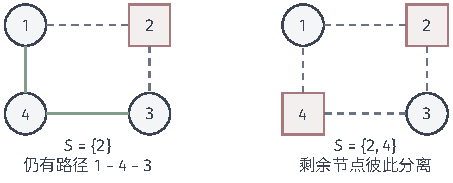
\includegraphics[width=76.652mm]{figures/06-probabilistic-graphical-models/01-representation/tikz/pgm-undirected-separation/figure.pdf}
  \caption{四节点环上的删除检测。方形节点属于条件集合$S$，与它们相接的虚线边一起删除，其余实线边保留。左侧只删$2$，仍可沿$1-4-3$连接；右侧删$2,4$，使$1,3$进入不同连通分量。}
  \label{fig:pgm-undirected-separation}
\end{figure}

\subsection{图分离的检测}
\label{sec:pgm-undirected-separation-test}

在$\mathcal{G}[V\setminus S]$中，从$A$的全部节点启动广度优先搜索，即可检查剩余连通性。搜索若到达$B$中的节点，就找到一条避开$S$的路径；若搜索结束仍未到达$B$，则$S$构成分离集。每次扩张都沿保留的节点和边进行，所以访问集恰好覆盖与$A$有剩余路径的节点，这给出算法的正确性依据。采用邻接表和标记数组时，最坏时间为$O(d+|E|)$，额外空间为$O(d)$。这一开销针对结构查询，概率数值计算还要处理模型的局部函数与状态汇总。

\subsection{图分离的可靠性与模型类完备性}
\label{sec:pgm-undirected-separation-soundness-completeness}

一个分离查询对应整类相容分布。\termalias{pgm-soundness}{可靠性}（soundness）要求图中读出的分离对该类每个分布都给出条件独立；\term{完备性}（completeness）则要求每项未分离查询至少有一个相容分布表现出依赖。前者作全称保证，后者构造存在见证，具体选定的参数仍可能产生额外独立。

为观察参数的作用，先构造一个由局部权重组成的分布。给局部变量组合的各状态指定非负权重，所得函数称为\term{势函数}（potential function），简称势。将一个完整配置涉及的权重相乘，再除以全部配置的权重总和，就得到概率。有限离散情形下，这个总和称为\term{配分函数}（partition function）$Z$，要求$Z>0$；归一化由全局总和完成，局部势只记录相对权重。

\begin{example}[不分离不强迫固定分布相关]
  \label{ex:pgm-undirected-fixed-distribution-extra-independence}
  考虑节点集$V=\{1,2\}$、边集$E=\{\{1,2\}\}$的无向图，并令$X_1,X_2\in\{-1,+1\}$。在唯一的二节点团上取常数边势
  \[
    \psi_{\{1,2\}}(x_1,x_2)=1.
  \]
  常数势给四个完整配置同样的权重$1$，总权重为$Z=1+1+1+1=4$。于是各配置的概率都是$p(x_1,x_2)=1/4$，得到一个严格正的联合分布。两个变量各自均匀取值，故对任意$x_1,x_2$，
  \[
    p(x_1,x_2)=\frac14
    =\frac12\cdot\frac12
    =p(x_1)p(x_2),
  \]
  即$X_1\perp X_2$。图中的边保留了两端发生相互作用的可能，常数势却没有使用这种相互作用。因而空集虽然无法分离两个端点，这组参数仍使二者独立。完备性要回答的是同一模型类中能否找到使二者依赖的参数；这个均匀分布只说明，选定参数可以带来图结构之外的独立性。
\end{example}

\begin{theorem}[团因子分解分布上的分离可靠性]
  \label{thm:pgm-undirected-factorization-to-global}
  设$\mathcal{G}=(V,E)$为有限简单无向图，节点$i\in V$取值于可测空间$(\mathcal{X}_i,\mathcal{A}_i)$，其上给定$\sigma$有限基准测度$\mu_i$；记$\mathcal{X}=\prod_{i\in V}\mathcal{X}_i$及$\mu=\bigotimes_{i\in V}\mu_i$，有限离散情形取计数测度。令$\mathcal{C}$为$\mathcal{G}$的有限团族，且对每个$C\in\mathcal{C}$，$\psi_C:\mathcal{X}_C\to[0,\infty)$是可测函数，其中$\mathcal{X}_C=\prod_{i\in C}\mathcal{X}_i$。若$p$相对于$\mu$的密度满足
  \[
    \begin{aligned}
      p(\bm{x})
      &=\frac{1}{Z}\prod_{C\in\mathcal{C}}\psi_C(\bm{x}_C)
        &&\text{$\mu$几乎处处},\\
      Z
      &=\int_{\mathcal{X}}\prod_{C\in\mathcal{C}}
        \psi_C(\bm{x}_C)\,\mathrm{d}\mu(\bm{x}),
        &&0<Z<\infty,
    \end{aligned}
  \]
  则对任意两两不交且$A,B$非空的$A,B,S\subseteq V$，若$S$在$\mathcal{G}$中分离$A$与$B$，就有
  \[
    \bm{X}_A\perp\bm{X}_B\mid\bm{X}_S.
  \]
  势函数可以取零，不要求$p$严格为正。
\end{theorem}

图中的分离使团势落在条件集的两侧；分别归一化这两组势，再消去$A\cup B\cup S$以外的变量，就能得到条件概率的乘积。第~\ref{sec:pgm-undirected-factorization-to-markov}节给出定理~\ref{thm:pgm-undirected-factorization-to-global}的完整证明。下面先沿着一条未被阻断的路径构造依赖，证明模型类的完备性。

\Needspace{14\baselineskip}
\begin{theorem}[严格正二值成对势模型类中的分离完备性]
  \label{thm:pgm-undirected-separation-completeness}
  设$\mathcal{G}=(V,E)$为有限简单无向图，每个节点$i\in V$对应二值随机变量$X_i\in\{-1,+1\}$，且$A,B,S\subseteq V$两两不交、$A,B$非空。若$S$在$\mathcal{G}$中不分离$A$与$B$，则存在一个严格正且按$\mathcal{G}$分解的成对势模型
  \[
    p(\bm{x})=\frac{1}{Z}
      \prod_{\{i,j\}\in E}\psi_{\{i,j\}}(x_i,x_j),
    \qquad \psi_{\{i,j\}}(x_i,x_j)>0,
  \]
  使$\bm{X}_A\not\perp\bm{X}_B\mid\bm{X}_S$。
\end{theorem}

\begin{proof}
从$A$到$B$存在一条避开$S$的路径；去掉路径中重复的节点，可取简单路径
\[
  v_0-v_1-\cdots-v_m,
  \qquad v_0\in A,\quad v_m\in B.
\]
取任意$J\neq0$。对路径上的边设
\[
  \psi_{\{v_{r-1},v_r\}}(x_{v_{r-1}},x_{v_r})
  =\exp(Jx_{v_{r-1}}x_{v_r}),
  \qquad r=1,\ldots,m,
\]
其余边的势取常数$1$。这样只让选定路径传递相互作用。所有势严格为正，状态空间有限，故$0<Z<\infty$，所得联合分布属于定理要求的模型类。

路径外的变量仅出现在常数势中，因而独立且均匀；连接路径内外的边也没有引入额外作用。完整联合分布由路径分布和路径外的均匀分布相乘得到。由于$\bm{X}_S$都位于路径外，给定它的取值后，路径分布保持原样：对每个$\bm{s}$，
\[
  p(x_{v_0},\ldots,x_{v_m}\mid\bm{s})
  =\frac12\prod_{r=1}^{m}
    \frac{\exp(Jx_{v_{r-1}}x_{v_r})}{2\cosh J}.
\]

把路径分布按相邻节点写成转移概率后，初始状态均匀，每一步都保留相同的耦合。令$\rho=\tanh J\neq0$，相邻节点的条件均值满足
\[
  \mathbb{E}[X_{v_r}\mid X_{v_{r-1}}]
  =\rho X_{v_{r-1}}.
\]
沿路径逐次取条件期望，每经过一条边便多乘一个耦合系数，得到
\[
  \mathbb{E}[X_{v_0}X_{v_m}\mid\bm{X}_S=\bm{s}]
  =\rho^m\neq0,
  \qquad
  \mathbb{E}[X_{v_0}\mid\bm{s}]
  =\mathbb{E}[X_{v_m}\mid\bm{s}]=0.
\]
两个端点的条件均值都是零，而乘积的条件均值非零，因此给定$\bm{X}_S$后仍有依赖。若$\bm{X}_A\perp\bm{X}_B\mid\bm{X}_S$，从两侧各取一个分量便应得到$X_{v_0}\perp X_{v_m}\mid\bm{X}_S$，与上述计算矛盾。选定的非零耦合由此提供了完备性所需的见证分布；换成零耦合，即$J$取零，同一张图也能表示独立分布。
\end{proof}

\section{无向图中的因子分解}
\label{sec:pgm-undirected-factorization}

图中缺边和分离约束了变量间的依赖，具体配置的概率则需要由参数确定。无向图通过团上的非负权重描述局部相容关系，将它们相乘并归一化后得到联合分布。本节先说明团势的组织与计算，再证明这种分解如何对应前面的Markov性质。

\subsection{因子分解的定义}
\label{sec:pgm-undirected-factorization-definition}

沿用前面的局部权重，为图中每个选定团指定一个势：设$\mathcal{C}$是团的一个族，$\psi_C(\bm{x}_C)$是团$C$上的有限非负函数。将这些势相乘，若能找到$0<Z<\infty$使
\begin{equation}
  p(\bm{x})=\frac{1}{Z}\prod_{C\in\mathcal{C}}\psi_C(\bm{x}_C),
  \label{eq:pgm-undirected-factorization}
\end{equation}
则称$p$按照$\mathcal{G}$进行团因子分解。每个势的自变量来自一个团，实际取值可以只受其中部分变量影响；例如常数势完全不使用团内变量的状态。

在离散状态空间上，归一化需要遍历完整配置，将相乘后的权重累加：
\begin{equation}
  Z=\sum_{\bm{x}\in\mathcal{X}}\prod_{C\in\mathcal{C}}\psi_C(\bm{x}_C),
  \qquad
  \mathcal{X}=\prod_{i\in V}\mathcal{X}_i.
  \label{eq:pgm-undirected-partition}
\end{equation}
有限状态空间上，这个有限和给出有限的$Z$；只要至少一个配置权重非零，便有合法的概率分布。可数无限状态空间还需要求和级数收敛。势$\psi_C$记录相对权重，其自身的总和可以异于$1$。不同团共享变量，局部各自归一化后，相乘的函数仍需要全局归一化常数$Z$。

全局归一化的代价取决于怎样组织求和。若$d$个变量各有$q$个状态，式~\eqref{eq:pgm-undirected-partition}的直接枚举要计算$q^d$项：$20$个二值变量就有$2^{20}=1048576$种配置。链、树或树宽较小的图能让不同配置共享部分计算，从而降低相对于枚举的开销；精确推断章节将说明如何利用这种结构。

给定其余所有变量后，计算一个节点的条件分布只需局部求和。记未归一化权重为$w(\bm{x})=\prod_{C\in\mathcal C}\psi_C(\bm{x}_C)$，固定$\bm{x}_{-i}=\bm{x}_{V\setminus\{i\}}$，取$p(\bm{x}_{-i})>0$的条件事件。条件概率的分子与分母都带有同一个全局常数：
\begin{equation}
  \begin{aligned}
    p(x_i\mid\bm{x}_{-i})
      &=\frac{w(x_i,\bm{x}_{-i})/Z}
        {\sum_{a\in\mathcal X_i}w(a,\bm{x}_{-i})/Z}\\
      &=\frac{\prod_{C\ni i}\psi_C(\bm{x}_C)}
        {\sum_{a\in\mathcal X_i}
          \prod_{C\ni i}\psi_C(a,\bm{x}_{C\setminus\{i\}})}.
  \end{aligned}
  \label{eq:pgm-undirected-local-conditional}
\end{equation}
在这个比值中，$Z$和所有不含$i$的势都被约去，分母只保留涉及$X_i$的势。记号$\psi_C(a,\bm{x}_{C\setminus\{i\}})$表示将第$i$个变量置为$a$，其余坐标使用已给定的值。二值节点因此只需把两项权重归一化。这个简化利用了其余变量全部已知的条件；若只有少数证据，未观测变量仍需边缘化，通常会留下更大的求和。

任意团都包含于某个极大团，因此小团势可以乘入一个包含它的极大团势。给每个小团选择一次归属，就能将所有势整理为仅以极大团为索引的乘积，同时保持原来的联合分布。“按团分解”与“按极大团分解”由此表示同一分布族，参数组织可以不同。团的阶数则影响所能表示的作用：一般的三节点团势包含三者共同取值的影响，单点势与成对势的乘积未必能表示它。

当势严格为正时，可以把乘积改写为指数形式。令$\varepsilon_C=-\log\psi_C$，并定义\term{能量函数}（energy function）$E(\bm{x})=\sum_C\varepsilon_C(\bm{x}_C)$，便有
\[
  p(\bm{x})=Z^{-1}\exp[-E(\bm{x})].
\]
指数形式将相乘的相容权重改为相加的能量，较低能量对应较大权重。零势可记作$\varepsilon_C=+\infty$，以表示被禁止的配置；后面需要计算有限对数差分的证明则限于严格正势。

连续变量将求和换成积分。指定各坐标上的$\sigma$有限基准测度$\mu_i$，联合基准测度为$\mu=\bigotimes_{i\in V}\mu_i$，实数变量通常取Lebesgue测度；这是第~\ref{sec:pgm-directed-factor-definition}节采用的密度约定。可测势的乘积需要满足
\begin{equation}
  0<Z=\int_{\mathcal{X}}\prod_{C\in\mathcal{C}}
       \psi_C(\bm{x}_C)\,\mathrm{d}\mu(\bm{x})<\infty.
  \label{eq:pgm-undirected-continuous-partition}
\end{equation}
有限且正的积分使式~\eqref{eq:pgm-undirected-factorization}成为归一化密度。这里检查的是整个势乘积：一些单独不可积的势相乘后可以可积，而$\mathbb{R}^d$上的正的常数势乘积仍会有无穷积分。后面的高斯参数化将用精度矩阵的正定性具体表达这项全局条件。

\begin{example}[四节点环上的相容分数]
  \label{ex:pgm-undirected-cycle}
  令$X_i\in\{0,1\}$，四条边上的势相同：
  \[
    \psi_{\{i,j\}}(x_i,x_j)=
    \begin{cases}
      2,&x_i=x_j,\\
      1,&x_i\neq x_j.
    \end{cases}
  \]
  两端状态相同的一条边将权重乘以$2$，不同的边保持权重。对图~\ref{fig:pgm-undirected-factorization-example}中的$\bm{x}=(0,0,1,1)$，四个边势的乘积是$4$，用$Z=82$归一化便得到概率$2/41$。为计算这个常数，将配置按相同边数分类：沿环回到起点时，状态改变次数为偶数，相同边数因此只能是$4,2,0$。表~\ref{tab:pgm-undirected-cycle-weights}据此汇总全部$16$种配置。
  三类权重相加给出$Z=32+48+2=82$。全相同配置的概率为$p(0,0,0,0)=16/82=8/41$，交替配置的概率为$p(0,1,0,1)=1/82$。相容势由此明确了各配置的相对概率；这些数值只用于演示指定势后的计算。
\end{example}

\begin{figure}[htbp]
  \centering
  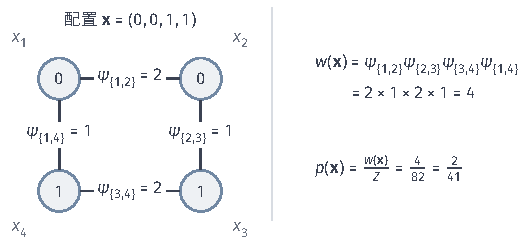
\includegraphics[width=89.701mm]{figures/06-probabilistic-graphical-models/01-representation/tikz/pgm-undirected-factorization-example/figure.pdf}
  \caption{四节点环中配置$\bm{x}=(0,0,1,1)$的权重与概率。四条边的势值相乘为$4$；全部$16$种配置的权重之和为$Z=82$，因此该配置的概率为$2/41$。}
  \label{fig:pgm-undirected-factorization-example}
\end{figure}

\begin{table}[htbp]
  \centering
  \begin{tabular}{crrr}
    \toprule
    相同边数 & 配置数 & 单个权重 & 总权重 \\
    \midrule
    $4$ & $2$ & $16$ & $32$ \\
    $2$ & $12$ & $4$ & $48$ \\
    $0$ & $2$ & $1$ & $2$ \\
    \bottomrule
  \end{tabular}
  \caption{按相同边数汇总四节点二值环的配置。相同边的势为$2$，不同边的势为$1$；各类总权重相加得到配分函数$82$。}
  \label{tab:pgm-undirected-cycle-weights}
\end{table}

\subsection{从因子分解到条件独立性}
\label{sec:pgm-undirected-factorization-to-markov}

删除分离集$S$后，图的连通分量将查询的两组节点隔开。团内节点两两相连，故一个团无法同时跨越这两侧。利用这一点整理团势，就能证明定理~\ref{thm:pgm-undirected-factorization-to-global}中的条件独立性。

\begin{proof}[定理~\ref{thm:pgm-undirected-factorization-to-global}的证明]
取两两不交且被$S$分离的$A,B,S$，其中$A,B$均非空。在$\mathcal{G}[V\setminus S]$中，将所有与$A$相交的连通分量合为$U$，其余节点合为$W=V\setminus(S\cup U)$。这些集合满足$A\subseteq U$、$B\subseteq W$，且$U$与$W$之间无边。

若一个团含有$U$和$W$各一个节点，两节点之间就应有边，这与集合的构造矛盾。因此每个团或者全部在$S$中，或者只涉及$U$与$S$，或者只涉及$W$与$S$。分别将这三类势相乘，联合分布写成
\begin{equation}
  p(\bm{u},\bm{w},\bm{s})
  =Z^{-1}h(\bm{s})f(\bm{u},\bm{s})g(\bm{w},\bm{s}),
  \label{eq:pgm-undirected-separated-factors}
\end{equation}
三组自变量$\bm{u},\bm{w},\bm{s}$分别对应$\bm{X}_U,\bm{X}_W,\bm{X}_S$；某类没有势时，其乘积取$1$。

为了将两侧函数归一化，在离散情形定义$F(\bm{s})=\sum_{\bm{u}}f(\bm{u},\bm{s})$、$G(\bm{s})=\sum_{\bm{w}}g(\bm{w},\bm{s})$；连续情形使用相应乘积测度的积分。取$p_S(\bm{s})$有限且严格为正的条件值，离散情形的所有正概率事件都满足此条件，连续情形中这样的取值承载全部$\bm{X}_S$概率。式~\eqref{eq:pgm-undirected-separated-factors}由此要求$h(\bm{s})$为正。团势非负，Tonelli定理允许先分别积分两侧函数，得到
\[
  p_S(\bm{s})=Z^{-1}h(\bm{s})F(\bm{s})G(\bm{s}).
\]
正且有限的条件密度排除了两侧积分为零或无穷的情形：$F(\bm{s})$或$G(\bm{s})$为零时联合积分为零，一侧积分无穷而另一侧为正时联合积分无穷。所以两侧的$F(\bm{s})$与$G(\bm{s})$均正且有限，条件联合密度成为
\begin{equation}
  p(\bm{u},\bm{w}\mid\bm{s})
  =\frac{f(\bm{u},\bm{s})}{F(\bm{s})}
   \frac{g(\bm{w},\bm{s})}{G(\bm{s})}.
  \label{eq:pgm-undirected-conditional-product}
\end{equation}
右侧各因子分别是两侧的条件密度，这个乘积给出$\bm{X}_U\perp\bm{X}_W\mid\bm{X}_S$。

最后分别消去$U\setminus A$和$W\setminus B$的变量。式~\eqref{eq:pgm-undirected-conditional-product}的两侧仍可独立求和或积分，留下只含$\bm{x}_A,\bm{s}$和只含$\bm{x}_B,\bm{s}$的条件边缘分布。故$\bm{X}_A\perp\bm{X}_B\mid\bm{X}_S$，任意被分离的两组变量都满足所需条件独立性。
\end{proof}

两侧函数的归一化在正概率条件事件或几乎处处的条件密度上完成，所除的常数正且有限。因此团势中的零值也适用于此证明。再结合定理~\ref{thm:pgm-undirected-global-implications}，团分解同时推出局部和成对性质。这个方向直接来自势乘积；下一节的Hammersley--Clifford结论负责相反方向，即从独立性重建团势。

对四节点环，可以直接看到这种两侧归一化。固定示例~\ref{ex:pgm-undirected-cycle}中的$X_2=x_2,X_4=x_4$，将涉及节点1和节点3的边势各自相乘：
\[
  \begin{aligned}
    f(x_1)&=\psi_{\{1,2\}}(x_1,x_2)\psi_{\{1,4\}}(x_1,x_4),\\
    g(x_3)&=\psi_{\{2,3\}}(x_2,x_3)\psi_{\{3,4\}}(x_3,x_4).
  \end{aligned}
\]
两邻居都取零时，即$x_2=x_4=0$，两侧权重满足$f(0)=g(0)=4$和$f(1)=g(1)=1$，因而
\[
  p(x_1,x_3\mid0,0)
  =\frac{1}{25}
    \begin{pmatrix}16&4\\4&1\end{pmatrix}_{x_1+1,x_3+1}.
\]
行与列都按状态$0,1$排列。两侧的条件边缘均为$(4/5,1/5)$，相乘正好得到矩阵的各项。若换成$x_2=0,x_4=1$，$f$与$g$的两种状态权重都为$2$，四个条件联合概率便都为$1/4$。两种条件值产生不同的边缘分布，但每种情况下，给定邻居后的联合分布都由两侧边缘相乘得到。

\subsection{从条件独立性到因子分解}
\label{sec:pgm-undirected-hammersley-clifford}

现在设联合分布满足图的独立性约束，需要为它找到团势。先选一个基准配置，将每次改变部分坐标引起的对数概率变化拆成局部作用；缺边所要求的条件独立性会让所有非团作用消失。下面采用Gill笔记中的构造完成这一逆向推导\scite{pgm-undirected-gill2011}

\term{Hammersley--Clifford定理}在有限离散、严格正的情形下给出独立性与团分解的等价关系。严格正的范围是完整的笛卡尔积$\mathcal{X}=\prod_i\mathcal{X}_i$：每个配置都须满足$p(\bm{x})>0$，包括尚未缩小为支持集时的所有组合。定理~\ref{thm:pgm-undirected-markov-equivalence}已证明三种Markov性质在这些条件下等价，所以只需从其中一种构造团势。

\begin{theorem}[有限离散Hammersley--Clifford定理]
  \label{thm:pgm-undirected-hammersley-clifford}
  设$\mathcal{G}=(V,E)$为有限简单无向图，每个节点$i\in V$对应取值于有限非空状态空间$\mathcal{X}_i$的随机变量$X_i$。令$p$为$\bm{X}=(X_i)_{i\in V}$在乘积状态空间$\mathcal{X}=\prod_{i\in V}\mathcal{X}_i$上的联合质量函数，并且$p(\bm{x})>0$对所有$\bm{x}\in\mathcal{X}$成立。则以下四个条件等价：$p$满足相对于$\mathcal{G}$的全局Markov性质；$p$满足相对于$\mathcal{G}$的局部Markov性质；$p$满足相对于$\mathcal{G}$的成对Markov性质；$p$能按$\mathcal{G}$的团分解。分解中的势可以全部取为严格正值。
\end{theorem}

\begin{proof}
团分解到全局性质的方向由定理~\ref{thm:pgm-undirected-factorization-to-global}给出，三种Markov性质的等价由定理~\ref{thm:pgm-undirected-markov-equivalence}给出。剩下的任务是从成对性质重建分布。任选基准配置$\bm{x}^{\circ}\in\mathcal{X}$，对每个$D\subseteq V$，记
\[
  \bm{x}^{D}=(\bm{x}_D,\bm{x}^{\circ}_{V\setminus D}),
  \qquad
  L_D(\bm{x}_D)=\log p(\bm{x}^{D}).
\]
配置只在$D$中的坐标使用当前值，其他坐标都取基准值。每个配置概率严格为正，所以这些对数可作为有限实数参与后面的加减。

为分离出每个坐标子集的作用，对每个$D\subseteq V$构造
\begin{equation}
  \phi_D(\bm{x}_D)
  =\sum_{B\subseteq D}(-1)^{|D|-|B|}L_B(\bm{x}_B).
  \label{eq:pgm-undirected-mobius}
\end{equation}
常数项为$\phi_{\varnothing}=\log p(\bm{x}^{\circ})$。这种\term{Möbius分解}（Möbius decomposition）用交替加减剔除较小子集的作用，留下同时改变$D$中各坐标时额外产生的部分。单节点项和二节点项分别为
\[
  \begin{aligned}
    \phi_{\{i\}}&=L_{\{i\}}-L_{\varnothing},\\
    \phi_{\{i,j\}}
      &=L_{\{i,j\}}-L_{\{i\}}-L_{\{j\}}+L_{\varnothing}.
  \end{aligned}
\]

验证这些局部项是否保留了完整分布，可将所有$D$的项重新相加。交换两层有限求和，得到
\begin{align}
  \sum_{D\subseteq V}\phi_D(\bm{x}_D)
  &=\sum_{B\subseteq V}L_B(\bm{x}_B)
      \sum_{D:\,B\subseteq D\subseteq V}(-1)^{|D|-|B|}
      \notag\\
  &=L_V(\bm{x}_V)=\log p(\bm{x}).
  \label{eq:pgm-undirected-mobius-inversion}
\end{align}
每个固定$B$对应的内层系数都是$(1-1)^{|V\setminus B|}$。$B\neq V$时该系数为零，$B=V$时剩下唯一一项$1$，所以最终仅保留完整配置的对数概率。

成对性质随后决定哪些局部项留下。非空子集$D$若不是团，其内就有不相邻节点$i,j$；令$R=V\setminus\{i,j\}$。固定任意$\bm{x}_R$时，两节点的条件联合概率由各自条件边缘相乘得到。因此对任意$a,a'\in\mathcal{X}_i$和$b,b'\in\mathcal{X}_j$，
\begin{equation}
  \begin{aligned}
    &p(a,b,\bm{x}_R)p(a',b',\bm{x}_R)\\
    &\qquad=p(a,b',\bm{x}_R)p(a',b,\bm{x}_R).
  \end{aligned}
  \label{eq:pgm-undirected-rectangle}
\end{equation}
等式两侧的条件归一化因子相同，约去后得到上述联合概率关系。取$a=x_i,a'=x_i^{\circ},b=x_j,b'=x_j^{\circ}$，使$R$中一个子集$B$使用当前值，其余坐标使用基准值。取有限对数后，有
\[
  L_{B\cup\{i,j\}}-L_{B\cup\{i\}}
  -L_{B\cup\{j\}}+L_B=0.
\]
这个零差分说明，其他坐标固定时，两非邻居的联合变化可以完全由各自的变化解释。

令$T=D\setminus\{i,j\}$。在式~\eqref{eq:pgm-undirected-mobius}中，按子集是否含有$i,j$将求和项分为四组，使每组对应刚才的一个矩形差分：
\begin{equation}
  \begin{aligned}
    \phi_D
    =\sum_{B\subseteq T}(-1)^{|T|-|B|}
      \bigl(&L_{B\cup\{i,j\}}-L_{B\cup\{i\}}\\
            &-L_{B\cup\{j\}}+L_B\bigr)=0.
  \end{aligned}
  \label{eq:pgm-undirected-nonclique-vanishes}
\end{equation}
每个括号都为零，故只要一个子集含有非邻接对，它的整个交互项就为零。这一步同时排除了涉及这对节点的所有更高阶项。

留下的非空子集全是团，记其族为$\mathcal{C}_{\mathrm{all}}$。令$\psi_C=\exp(\phi_C)>0$，将式~\eqref{eq:pgm-undirected-mobius-inversion}的和指数化，得到
\[
  p(\bm{x})
  =\exp(\phi_{\varnothing})
     \prod_{C\in\mathcal{C}_{\mathrm{all}}}\psi_C(\bm{x}_C).
\]
联合概率对$\bm{x}$求和为一，所以团势乘积的配分函数是$Z=\exp(-\phi_{\varnothing})$，正且有限。若需仅保留极大团，进一步将每个小团势并入一个包含它的极大团即可。
\end{proof}

Möbius恒等式负责重建对数概率，成对独立性负责消去非团项，两者共同给出团分解。严格正性使每个其余变量配置都能用于条件化，也使矩形等式的对数有限。这是逆向结论在整类分布上成立的充分条件。沿用四节点环，下面给出一个带零概率的分布：它满足所有Markov独立性，却无法按团分解，从而展示严格正性所保护的方向。

\begin{example}[满足全局Markov性质却不能团分解]
  \label{ex:pgm-undirected-zero-support}
  在同一四节点环上，用两个相互独立的公平二值变量$U,V$构造分布：
  \[
    X_1=U,\quad X_2=V,\quad
    X_3=U\mathbin{\oplus}V,\quad X_4=U,
  \]
  $\oplus$表示模$2$加法。两变量的四种取值分别生成表~\ref{tab:pgm-undirected-zero-support}中的四个配置，其他完整配置的概率均为零。
\end{example}

\begin{table}[htbp]
  \centering
  \begin{tabular}{ccccc}
    \toprule
    $x_1$ & $x_2$ & $x_3$ & $x_4$ & 概率 \\
    \midrule
    $0$ & $0$ & $0$ & $0$ & $1/4$ \\
    $0$ & $1$ & $1$ & $0$ & $1/4$ \\
    $1$ & $0$ & $1$ & $1$ & $1/4$ \\
    $1$ & $1$ & $0$ & $1$ & $1/4$ \\
    \bottomrule
  \end{tabular}
  \caption{四节点环中四个正概率配置。给定任意一对对角节点即可确定所在行；边上的取值对允许的组合则多于这个全局支持集。}
  \label{tab:pgm-undirected-zero-support}
\end{table}

先检验独立性。给定$(X_2,X_4)$便知道$(U,V)$，$X_1$与$X_3$都成为常量，所以二者条件独立。给定$(X_1,X_3)$也能确定$(U,V)$，从而$X_2\perp X_4\mid(X_1,X_3)$。四节点环删除一个节点仍连通，非空节点集间的非平凡分离只可能是用一对对角节点隔开另一对。这两项条件独立因此覆盖全局Markov性质要求的所有查询，局部和成对性质也随之成立。

再检验能否分解。假设已有四个边势，单点势可先乘入某个关联的边势。取零概率配置$\bm{y}=(0,0,1,0)$：边$\{1,2\}$的取值$(0,0)$在正概率配置$(0,0,0,0)$中出现；边$\{2,3\}$的取值$(0,1)$在$(1,0,1,1)$中出现；边$\{3,4\}$的取值$(1,0)$在$(0,1,1,0)$中出现；边$\{1,4\}$的取值$(0,0)$则又在$(0,0,0,0)$中出现。每个正概率配置都要求其边势乘积为正，所以上述四个边势值全部为正。在$\bm{y}$处相乘便会给出$p(\bm{y})>0$，与指定的零概率矛盾。

图~\ref{fig:pgm-undirected-zero-support}将这四个取值对标在环的边上。局部投影各自允许这些取值，拼成的完整配置却不属于表~\ref{tab:pgm-undirected-zero-support}的支持集。
\begin{figure}[htbp]
  \centering
  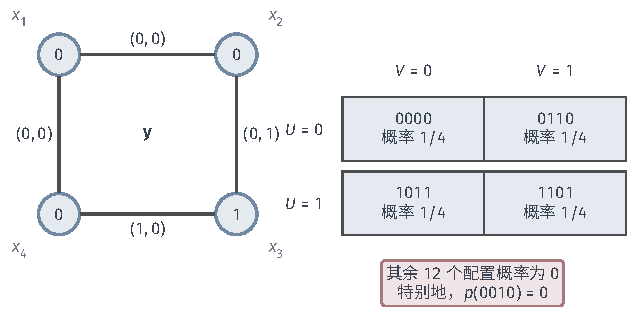
\includegraphics[width=106.825mm]{figures/06-probabilistic-graphical-models/01-representation/tikz/pgm-undirected-zero-support/figure.pdf}
  \caption{全局Markov性质成立而团分解失败的零概率反例。左侧配置$\bm y=(0,0,1,0)$的每个边取值对都出现在正概率配置中；右侧$2\times2$表按$(U,V)$列出四个正概率配置，其余12个配置的概率为0。边势若表示这些正概率配置，$\bm y$处的各势值也须为正，故无法同时满足$p(\bm y)=0$。}
  \label{fig:pgm-undirected-zero-support}
\end{figure}

这个分布的条件独立来自条件变量对其余变量的完全确定。其全局支持约束却超出了边势能表达的范围：四个局部允许的取值对可以拼成一个全局禁止的配置。上述矛盾直接排除了非负团势分解。零概率分布中也有可分解的情形，例如边势$\mathbf{1}\{x_i=x_j\}$能用局部零值施加相等约束；有零值时，逆向分解是否成立取决于具体支持结构。

对连续密度，基准配置构造还遇到逐点值的问题。若只知道$p>0$几乎处处，一个预先固定的坐标截面可能属于零测集，而密度在这样的集合上可任意修改。这会影响在截面上定义$L_D$的逐点推理。一般可测空间中的逆向定理需要处理这些例外集合及密度版本\scite{pgm-lauritzen1996}

连续性可提供一个便于核验的充分条件。令$\mathcal{X}=\prod_i I_i$，其中$I_i$均为非空开区间，取Lebesgue乘积测度；设$p$连续、处处严格正，且积分为$1$。满足成对Markov性质时，存在连续严格正的团势，其乘积等于$p$乘以一个有限正数。为证明这一点，先由条件独立性得到式~\eqref{eq:pgm-undirected-rectangle}对$(a,a',b,b',\bm{x}_R)$几乎处处成立。两侧之差连续，若有一点非零，便会在该点某个正测度邻域中非零，与几乎处处相等矛盾。矩形等式因而处处成立，可以选取任意域内基准配置，再应用有限节点集合的Möbius分解。团势乘积与$p$成正比例，可积性也随之得到保证。

上述连续性只用于将几乎处处的矩形等式推广为逐点等式，一般可测版本可以采用其他条件。若要进一步利用$\log p$的混合偏导，则还需相应的可微性，例如二阶连续可微。实际建模时选定光滑势或神经参数化势后，也须检查整个乘积的可积性；存在某组团函数的分解定理，并未替具体函数族及参数完成这项检查。

\section{局部参数化}
\label{sec:pgm-undirected-local-parameterization}

为图中的团选定势函数，就得到可用于计算和学习的模型。离散变量可以使用表格或配置特征，连续变量可以使用二次函数等形式；每种参数化都需让全局归一化常数正且有限。

\subsection{离散变量的局部参数化}
\label{sec:pgm-undirected-discrete-parameterization}

以离散状态的偏好为例，单点势$\psi_{\{i\}}(x_i)$给每个状态指定权重，成对势$\psi_{\{i,j\}}(x_i,x_j)$给状态对指定相容权重，高阶势则记录多个状态组合的额外作用。最直接的表示是势表；每个变量有$q$个状态时，一般的$k$节点团需要$q^k$个表项。增加团的阶数能容纳更丰富的共同作用，也相应增加存储量。

若势严格为正，还可用团内特征$f_{C,r}(\bm{x}_C)$表示它的对数。选择“两个状态相同”或“团取某个配置”等指示特征后，为每个特征指定一个系数：
\[
  \log\psi_C(\bm{x}_C;\bm{\theta})
  =\sum_r\theta_{C,r}f_{C,r}(\bm{x}_C).
\]
将各团特征与系数分别汇总为$\bm{f}(\bm{x})$和$\bm{\theta}$，势乘积就对应特征内积的指数，形成\term{对数线性模型}（log-linear model）：
\begin{equation}
  \begin{aligned}
    p_{\bm{\theta}}(\bm{x})
      &=\exp\{\bm{\theta}^{\top}\bm{f}(\bm{x})-A(\bm{\theta})\},\\
    A(\bm{\theta})
      &=\log\sum_{\bm{x}}
          \exp\{\bm{\theta}^{\top}\bm{f}(\bm{x})\}.
  \end{aligned}
  \label{eq:pgm-undirected-exponential-family}
\end{equation}
参数通过特征内积进入指数，归一化由$A=\log Z$完成，故该模型属于\term{指数族}（exponential family）。为每个团配置都设置一个指示特征，可以表示任意严格正的团势表；减少特征或让多处特征共享系数，可以节省参数，同时缩小图结构允许的分布族\scite{pgm-wainwright2008}

\term{Ising模型}用$x_i\in\{-1,+1\}$表示两个状态，分别以状态值和相邻状态乘积为特征：
\begin{equation}
  p(\bm{x})=\frac{1}{Z}
  \exp\left\{\sum_i h_i x_i+
             \sum_{\{i,j\}\in E}J_{i,j}x_i x_j\right\}.
  \label{eq:pgm-undirected-ising}
\end{equation}
单点系数$h_i>0$提高$+1$状态的权重，边系数$J_{i,j}>0$提高相同状态对的权重，$J_{i,j}<0$则提高不同状态对的权重。这些系数控制对数相容分数，边缘概率还由其余势及全局归一化共同确定。把示例~\ref{ex:pgm-undirected-cycle}的状态通过$s_i=2x_i-1$换为$\{-1,+1\}$，原来的边势可写成
\[
  \psi_{\{i,j\}}(x_i,x_j)
  =\sqrt{2}\exp\left\{\frac{\log2}{2}s_i s_j\right\}.
\]
四条边的$\sqrt{2}$相乘只产生一个常数，可并入$Z$。因此该例对应单点系数为零、边耦合为$J_{i,j}=(\log2)/2$的Ising环。

当状态数增加为$x_i\in\{1,\ldots,q\}$时，\term{Potts模型}可用类别是否相同作为特征，其常见边势为
\[
  \psi_{\{i,j\}}(x_i,x_j)
  =\exp\{J_{i,j}\mathbf{1}\{x_i=x_j\}\}.
\]
类别编号只用于区分状态，势通过是否相同来奖励或惩罚组合，无需定义类别间的数值距离。更高阶的特征还可表达共同作用：对三个取值为$\{-1,+1\}$的变量，三节点团中的对数势$\lambda x_i x_j x_k$能区分乘积为正与为负的配置。使用该特征需要相应的团结构；在不含该团的图上增加这样的势，一般会改变原来的独立性约束。第~\ref{chap:pgm-energy-models}章继续讨论Ising、Potts及其他能量模型的建模和计算。

从数据估计这些系数时，全局归一化进入了优化目标。给定$n$个完整、独立同分布的样本向量$\bm{x}_1,\ldots,\bm{x}_n$，以$\overline{\bm{f}}=n^{-1}\sum_{k=1}^n\bm{f}(\bm{x}_k)$表示经验特征均值，平均对数似然及梯度为
\begin{equation}
  \begin{aligned}
    \ell(\bm{\theta})
      &=\bm{\theta}^{\top}\overline{\bm{f}}-A(\bm{\theta}),\\
    \nabla_{\bm{\theta}}\ell(\bm{\theta})
      &=\overline{\bm{f}}
        -\mathbb{E}_{p_{\bm{\theta}}}[\bm{f}(\bm{X})].
  \end{aligned}
  \label{eq:pgm-undirected-learning-gradient}
\end{equation}
梯度的第二项来自归一化函数对参数的导数，可由有限和中的指数逐项求导得到。它要求将数据中的特征平均与当前联合分布中的特征期望比较，参数学习因此反复调用推断。式~\eqref{eq:pgm-undirected-local-conditional}的单节点条件归一化解决的是给定其余变量的查询，这里的期望则针对整个联合分布。树上可通过消息计算，一般图的开销取决于消元所形成的中间因子。第~\ref{chap:pgm-elimination}章介绍这类推断，第~\ref{chap:pgm-parameter-learning}章进一步说明它在参数估计中的作用。

\subsection{连续变量的局部参数化}
\label{sec:pgm-undirected-continuous-parameterization}

对连续变量，二次能量提供了可精确计算的局部参数化，其系数还决定势乘积能否在全空间归一化。\term{高斯Markov随机场}（Gaussian Markov random field, GMRF）用无向图表示联合高斯分布的条件独立性。先考虑$\mathbb{R}^d$上相对于Lebesgue测度的非退化分布，令
\begin{equation}
  \begin{aligned}
    p(\bm{x})&=Z^{-1}
      \exp\left\{-\tfrac12\bm{x}^{\top}\bm{Q}\bm{x}
                   +\bm{h}^{\top}\bm{x}\right\},\\
    \bm{Q}&=\bm{Q}^{\top}\succ0.
  \end{aligned}
  \label{eq:pgm-undirected-gaussian}
\end{equation}
$\bm{Q}$称为\term{精度矩阵}（precision matrix），是协方差矩阵的逆；$\bm{h}\in\mathbb{R}^d$控制线性项。将指数中的二次式配方，可读取均值$\bm{m}=\bm{Q}^{-1}\bm{h}$与协方差$\bm{\Sigma}=\bm{Q}^{-1}$，积分得到
\begin{equation}
  Z=(2\pi)^{d/2}\det(\bm{Q})^{-1/2}
     \exp\left\{\tfrac12\bm{h}^{\top}\bm{Q}^{-1}\bm{h}\right\}.
  \label{eq:pgm-undirected-gaussian-partition}
\end{equation}
正定性让各方向的二次项都将密度压向有限区域，因而积分有限。对于这种全空间二次能量，它也是必要条件。将坐标轴变换到$\bm{Q}$的特征向量方向后，负特征值会让指数沿相应方向按正二次项增长；零特征值则只留下线性指数或常数。在整条实轴上，这两种情形的积分都发散。

展开二次型，就能将单节点项与节点对的作用分开：
\[
  \begin{aligned}
    &-\tfrac12\bm{x}^{\top}\bm{Q}\bm{x}+\bm{h}^{\top}\bm{x}\\
    &\qquad=\sum_i\left(-\tfrac12 Q_{i,i}x_i^2+h_i x_i\right)
             -\sum_{i<j}Q_{i,j}x_i x_j.
  \end{aligned}
\]
记$Q_{i,j}$为$\bm{Q}$的第$(i,j)$个元素。单点项指数化后成为单点势，非零交叉项则成为边势$\exp(-Q_{i,j}x_i x_j)$。这个边势单独可能不可积，其用途是参与全局势乘积，后者由正定性保证可积。所有缺边都满足$Q_{i,j}=0$时，交叉项仅出现在图的边上，得到所需团分解。

非退化高斯分布中，精度的非对角零元恰好对应成对条件独立性：
\begin{equation}
  Q_{i,j}=0
  \quad\Longleftrightarrow\quad
  X_i\perp X_j\mid\bm{X}_{V\setminus\{i,j\}},
  \qquad i\neq j.
  \label{eq:pgm-undirected-precision-independence}
\end{equation}
固定其余坐标，$(X_i,X_j)$的条件分布仍为高斯，其二次项的精度是主子矩阵
\[
  \begin{pmatrix}Q_{i,i}&Q_{i,j}\\Q_{i,j}&Q_{j,j}\end{pmatrix}.
\]
该矩阵正定，故$Q_{i,i}Q_{j,j}-Q_{i,j}^2>0$。求这个$2\times2$矩阵的逆，条件协方差的非对角元素为
\[
  -\frac{Q_{i,j}}{Q_{i,i}Q_{j,j}-Q_{i,j}^2}.
\]
两个高斯分量独立当且仅当协方差为零，上述非对角元素又恰在精度非对角元素为零时消失，得到式~\eqref{eq:pgm-undirected-precision-independence}。这里的查询包含其余全部变量作为条件。相比之下，$\Sigma_{i,j}=0$给出边缘独立性，$Q_{i,j}=0$给出条件独立性；两种矩阵的稀疏结构回答不同的问题。

若只留下第$i$个坐标，将涉及$x_i$的项配方，就得到单节点条件分布
\begin{equation}
  X_i\mid\bm{x}_{V\setminus\{i\}}
  \sim\mathcal{N}\left(
    \frac{h_i-\sum_{j\neq i}Q_{i,j}x_j}{Q_{i,i}},
    \frac{1}{Q_{i,i}}\right).
  \label{eq:pgm-undirected-gaussian-conditional}
\end{equation}
非邻居的精度系数为零，因而条件均值只用到邻居。反过来，若先指定每个节点的高斯条件分布，其参数就须与同一个联合精度匹配。给定条件方差$1/\tau_i$和条件均值$\alpha_i+\sum_{j\neq i}\beta_{i,j}x_j$，匹配上式需要$Q_{i,i}=\tau_i$、$Q_{i,j}=-\tau_i\beta_{i,j}$以及$h_i=\tau_i\alpha_i$。因此$\tau_i\beta_{i,j}=\tau_j\beta_{j,i}$保证$\bm{Q}$对称，整个$\bm{Q}$还须正定。所有$\tau_i>0$只保证各条件方差为正；这些局部合法的条件分布还要满足上述兼容条件，才构成所要求的联合高斯分布\scite{pgm-undirected-rue2005}

仍以四节点环为例，令$\bm{h}=\bm{0}$，选精度矩阵
\[
  \bm{Q}=
  \begin{pmatrix}
    3&-1&0&-1\\
    -1&3&-1&0\\
    0&-1&3&-1\\
    -1&0&-1&3
  \end{pmatrix}.
\]
用该环的图Laplacian矩阵$\bm{L}$表示时，其对角元素为节点度数，相邻处为$-1$，其他元素为$0$，于是$\bm{Q}=\bm{I}+\bm{L}$。对任意非零$\bm{v}$，
\[
  \bm{v}^{\top}\bm{Q}\bm{v}
  =\sum_i v_i^2+\sum_{\{i,j\}\in E}(v_i-v_j)^2>0,
\]
二次型严格为正，保证了这个精度对应合法密度。求逆得到协方差矩阵
\[
  \bm{\Sigma}=\frac{1}{15}
  \begin{pmatrix}
    7&3&2&3\\
    3&7&3&2\\
    2&3&7&3\\
    3&2&3&7
  \end{pmatrix}.
\]
两矩阵在同一位置给出$Q_{1,3}=0$与$\Sigma_{1,3}=2/15$，因此两对角节点边缘相关，给定另外两节点后独立。具体到节点$1$，条件均值为$(x_2+x_4)/3$，条件方差为$1/3$，不随$x_3$变化。它与离散环共享同一组图分离关系，条件分布的形式则由高斯参数化确定。

若将上例的$\bm{Q}$换为$\bm{L}$，情况便不同。令$\bm{1}$为全$1$向量，有$\bm{L}\bm{1}=\bm{0}$；同时平移全部坐标时能量不变，积分沿常数方向发散。这种奇异半正定精度在$\mathbb{R}^d$上无法产生非退化的归一化密度。\term{内蕴高斯Markov随机场}（intrinsic GMRF）使用的正是这类未完全归一化的模型。可在适当子空间上加约束、指定相应测度来构造分布，或在合适条件下结合似然得到可归一化的后验；这些处理需要各自的归一化论证，式~\eqref{eq:pgm-undirected-gaussian-partition}要求的可逆正定精度已不适用。子空间上的退化高斯也须重新判断条件独立性。

预测任务还可将已知输入用于确定势函数。以$\bm{x}$表示输入、$\bm{y}$表示待预测输出，\term{条件Markov网络}（conditional Markov network）定义输出的条件分布：
\begin{equation}
  p_{\bm{\theta}}(\bm{y}\mid\bm{x})
  =\frac{1}{Z_{\bm{\theta}}(\bm{x})}
    \prod_{C\in\mathcal{C}}
    \psi_C(\bm{y}_C;\bm{x},\bm{\theta}).
  \label{eq:pgm-undirected-conditional-network}
\end{equation}
图的节点只对应输出变量，固定的$\bm{x}$可以影响每个势。归一化对$\bm{y}$求和或积分，且每个使用的输入都需满足$0<Z_{\bm{\theta}}(\bm{x})<\infty$；输入本身的联合分布留在这个模型之外。输出可为离散或连续状态，高斯输出相应要求$\bm{Q}(\bm{x})$在每个允许输入下对称正定。第~\ref{chap:pgm-energy-models}章将介绍条件随机场等具体模型。

一个势的参数虽然只涉及局部变量，更新它通常会改变$Z$，从而改变许多配置的概率，影响也可能传至远处变量的边缘分布。另一方面，同一联合分布可以有多组势表示：势乘以正常数后可由$Z$吸收；两个共享节点的团还可将同一个正函数乘入一侧、从另一侧除去，保持总乘积不变。若估计任务要求参数唯一，就需为这些自由度另设约定。

表示与计算还要共同考虑图的规模和结构。高阶团增加势表大小，环可能让消元形成比原始团更大的中间团。四节点环可以直接枚举核算，大图的中间因子则可能成为主要成本。高斯参数化将积分化为线性方程求解与行列式计算，稠密情形通常需$O(d^3)$量级运算；稀疏结构的收益取决于消元中产生的填充。选择势表、二次能量或输入依赖势时，所需的表达能力、全局归一化条件及查询成本共同决定合适的参数化。

\section{本章小结}
\label{sec:pgm-undirected-summary}

无向图通过路径分离表达条件独立性。全局、局部与成对Markov性质分别从集合分离、邻居Markov毯和缺边描述这种约束；对一般分布，全局性质推出局部性质，局部性质再推出成对性质。团势乘积在分离集两侧分别归一化后成为条件概率的乘积，因此团分解推出全局性质，势中的零值也允许保留。

在有限离散严格正的情形，Möbius分解从对数概率中分离各子集的作用，成对独立性使非团项消失，由此得到Hammersley--Clifford逆向结论。零支持反例展示了该方向在去掉严格正性后的失效情形，连续密度则还需处理测度、密度版本与可积性。具体模型的势决定局部相容关系，配分函数完成全局归一化；离散特征和高斯精度分别实现不同的参数化，也带来不同的推断代价。下一章据此比较有向图、无向图与因子图的表示及转换，见第~\ref{chap:pgm-representations}章。

\paragraph{扩展阅读}
Lauritzen的教材系统讨论图分离、Markov性质与因子分解，适合进一步考察逆向结论的严格正条件；Bishop的PRML第8章用具体图结构解释这些关系。结合本章的势乘积计算，可从两书中的例子继续研究势函数尺度的自由度与配分函数的作用\scite{pgm-lauritzen1996,bishop2006}
